\documentclass[12pt,letterpaper]{article}

\usepackage{amsmath}
\usepackage{fontspec}
\setromanfont[Ligatures=TeX]{TeX Gyre Pagella}
\usepackage{unicode-math}
\setmathfont{TeX Gyre Pagella Math}
\usepackage[title]{appendix}
\usepackage[margin=1.0in]{geometry}
\usepackage[figuresleft]{rotating}
\usepackage[longnamesfirst]{natbib}
\usepackage{dcolumn}
\usepackage{booktabs}
\usepackage{multirow}
\usepackage[flushleft]{threeparttable}
\usepackage{setspace}
\usepackage[justification=centering,skip=2pt]{caption}
\usepackage[font=scriptsize]{subfig}
\usepackage[xetex,colorlinks=true,linkcolor=black,citecolor=black,urlcolor=black]{hyperref}
\usepackage{adjustbox}
\usepackage{xfrac}
\usepackage{placeins}

% For word counting uncomment line below and raggedright below
% http://countwordsfree.com/#
% \usepackage[nolists]{endfloat}


% \bibpunct{(}{)}{;}{a}{}{,}
\newcommand{\mco}[1]{\multicolumn{1}{c}{#1}}
\newcommand{\mct}[1]{\multicolumn{2}{c}{#1}}
\newcommand{\mcth}[1]{\multicolumn{3}{c}{#1}}
\newcommand{\X}{$\times$ }
\newcommand{\hs}{\hspace{15pt}}

% Attempt to squeeze more floats in
\renewcommand\floatpagefraction{.9}
\renewcommand\topfraction{.9}
\renewcommand\bottomfraction{.9}
\renewcommand\textfraction{.1}
\setcounter{totalnumber}{50}
\setcounter{topnumber}{50}
\setcounter{bottomnumber}{50}


%------------------------------------------------------------------------


\title{Birth Spacing and Fertility in the Presence of Son Preference and Sex-Selective Abortions:
India's Experience Over Four Decades \bigskip

Online Appendices 
}

\author{Claus C P\"ortner\\
    Department of Economics\\
    Albers School of Business and Economics\\
    Seattle University, P.O. Box 222000\\
    Seattle, WA 98122\\
    \href{mailto:cportner@seattleu.edu}{\texttt{cportner@seattleu.edu}}\\
    \href{http://www.clausportner.com}{\texttt{www.clausportner.com}}\\
    \& \\
    Center for Studies in Demography and Ecology \\
    University of Washington\\ \vspace{2cm}
    }

\date{Text and code for this paper are available at 
\href{https://github.com/cportner/sexSelectionSpacing}{https://github.com/cportner/sexSelectionSpacing}
}




%------------------------------------------------------------------------


\begin{document}
\graphicspath{{../figures/}}
\DeclareGraphicsExtensions{.eps,.jpg,.pdf,.mps,.png}

\setcounter{page}{0}
\maketitle
\thispagestyle{empty}

\section*{Appendices for Online Publication}

These appendices are intended for online publication.
They provide the descriptive statistics, additional
estimated duration tables, and graphs for all 
education groups and spells.

\clearpage
\newpage

\appendix

% CHANGING NUMBERING OF FIGURES AND TABLES FOR APPENDIX
\renewcommand\thefigure{\thesection.\arabic{figure}}    
\renewcommand\thetable{\thesection.\arabic{table}}    


\section{Characteristics of Women's Work Experiences}


\setcounter{figure}{0}
\setcounter{table}{0}

Figure \ref{fig:work_by_survey} shows the percent of married women who are 
currently working at the time of the survey by age group and education level.
No other labor force participation question is consistently available across all 
four surveys. 
Because the question refers to currently working, the percentages are lower in previous
studies. 

\captionsetup[figure]{skip = 10pt}

\begin{figure}[!htpb]
\centering
\rotatebox[origin=c]{90}{\small{40 Years or Older}}
\subfloat[Rural]{
    \begin{minipage}{0.4\textwidth}
        \includegraphics[width=\textwidth]{currently_working_rural_40}
    \end{minipage}
} 
\subfloat[Urban]{
    \begin{minipage}{0.4\textwidth}
        \includegraphics[width=\textwidth]{currently_working_urban_40} 
    \end{minipage}
}
\\
\rotatebox[origin=c]{90}{\small{30--39 Years Old}}
\subfloat[Rural]{
    \begin{minipage}{0.4\textwidth}
        \includegraphics[width=\textwidth]{currently_working_rural_30}
    \end{minipage}
} 
\subfloat[Urban]{
    \begin{minipage}{0.4\textwidth}
        \includegraphics[width=\textwidth]{currently_working_urban_30} 
    \end{minipage}
}
\\
\rotatebox[origin=c]{90}{\small{20--29 Years Old}}
\subfloat[Rural]{
    \begin{minipage}{0.4\textwidth}
        \includegraphics[width=\textwidth]{currently_working_rural_20}
    \end{minipage}
} 
\subfloat[Urban]{
    \begin{minipage}{0.4\textwidth}
        \includegraphics[width=\textwidth]{currently_working_urban_20} 
    \end{minipage}
}
\caption{Percentage of married women who were working at the time of the 
survey by age group and area of residence}
\label{fig:work_by_survey}
\end{figure}


\begin{figure}[!htpb]
\centering
\rotatebox[origin=c]{90}{\small{40 Years or Older}}
\subfloat[Rural]{
    \begin{minipage}{0.4\textwidth}
        \includegraphics[width=\textwidth]{work_cash_rural_40}
    \end{minipage}
} 
\subfloat[Urban]{
    \begin{minipage}{0.4\textwidth}
        \includegraphics[width=\textwidth]{work_cash_urban_40} 
    \end{minipage}
}
\\
\rotatebox[origin=c]{90}{\small{30--39 Years Old}}
\subfloat[Rural]{
    \begin{minipage}{0.4\textwidth}
        \includegraphics[width=\textwidth]{work_cash_rural_30}
    \end{minipage}
} 
\subfloat[Urban]{
    \begin{minipage}{0.4\textwidth}
        \includegraphics[width=\textwidth]{work_cash_urban_30} 
    \end{minipage}
}
\\
\rotatebox[origin=c]{90}{\small{20--29 Years Old}}
\subfloat[Rural]{
    \begin{minipage}{0.4\textwidth}
        \includegraphics[width=\textwidth]{work_cash_rural_20}
    \end{minipage}
} 
\subfloat[Urban]{
    \begin{minipage}{0.4\textwidth}
        \includegraphics[width=\textwidth]{work_cash_urban_20} 
    \end{minipage}
}
\caption{Percentage of women paid cash or cash and in-kind of those women who were 
working at the time of the survey by age group and area of residence}
\label{fig:work_cash_by_survey}
\end{figure}



\begin{figure}[!htpb]
\centering
\rotatebox[origin=c]{90}{\small{40 Years or Older}}
\subfloat[Rural]{
    \begin{minipage}{0.4\textwidth}
        \includegraphics[width=\textwidth]{work_family_rural_40}
    \end{minipage}
} 
\subfloat[Urban]{
    \begin{minipage}{0.4\textwidth}
        \includegraphics[width=\textwidth]{work_family_urban_40} 
    \end{minipage}
}
\\
\rotatebox[origin=c]{90}{\small{30--39 Years Old}}
\subfloat[Rural]{
    \begin{minipage}{0.4\textwidth}
        \includegraphics[width=\textwidth]{work_family_rural_30}
    \end{minipage}
} 
\subfloat[Urban]{
    \begin{minipage}{0.4\textwidth}
        \includegraphics[width=\textwidth]{work_family_urban_30} 
    \end{minipage}
}
\\
\rotatebox[origin=c]{90}{\small{20--29 Years Old}}
\subfloat[Rural]{
    \begin{minipage}{0.4\textwidth}
        \includegraphics[width=\textwidth]{work_family_rural_20}
    \end{minipage}
} 
\subfloat[Urban]{
    \begin{minipage}{0.4\textwidth}
        \includegraphics[width=\textwidth]{work_family_urban_20} 
    \end{minipage}
}
\caption{Percentage women who worked for a family member of those 
working at the time of the survey, by age group and area of residence}
\label{fig:work_family_by_survey}
\end{figure}


\clearpage
\newpage

\section{Empirical Model Details}

\setcounter{figure}{0}
\setcounter{table}{0}

% [More formal version of empirical strategy section]


The model is a discrete time, nonproportional, competing risk hazard model with two exit 
states: Either a boy or a girl is born.
The unit of analysis is a spell, the period from nine months after one birth to the next.
For each woman, $i=1,\ldots,n$, the starting point for a spell is time $t=1$, and 
the spell continues until time $t_i$, when either a birth occurs or the spell 
is censored.%
\footnote{
The time of censoring is assumed independent of the hazard rate,
as is standard in the literature.
}
There are two exit states: The birth of a boy, $j=1$, or the birth of a girl, $j=2$, and 
$J_i$ is a random variable indicating which event took place.
The discrete time hazard rate $h_{ijt}$ is 
\begin{equation}
 h_{ijt} = \frac{\exp(D_j(t) + \alpha_{jt}'\mathbf{Z}_{it} + \beta_j'\mathbf{X}_{i})} 
 {1 + \sum_{l=1}^2 \exp(D_j(t) + \alpha_{lt}'\mathbf{Z}_{it} + \beta_l'\mathbf{X}_{i})} \: \: \; \; \;  j = 1,2
 \label{eq:hazard_appendix}
\end{equation}
where the explanatory variable vectors, $\mathbf{Z}_{it}$ and $\mathbf{X}_{i}$, capture 
individual, household, and community characteristics,
and $D_{j}(t)$ is the piece-wise linear baseline hazard for outcome $j$, captured
by dummies and the associated coefficients,
\begin{equation}
D_j(t) = \gamma_{j1} D_1 + \gamma_{j2} D_2 + \ldots + \gamma_{jT} D_T,
\end{equation}
with $D_m = 1$ if $t=m$ and zero otherwise.
This approach to modeling the baseline hazard is flexible and does not place 
overly strong restrictions on the baseline hazard.

The explanatory variables in $\mathbf{Z}$, and the interactions between them, 
constitute the nonproportional part of the model, which means that they are
interacted with the baseline hazard:
\begin{equation}
 \mathbf{Z}_{it} = D_j(t) \times (\mathbf{Z}_1 + Z_2 + \mathbf{Z}_1 \times Z_2),
\end{equation}
where $D_j(t)$ is the piece-wise linear baseline hazard, $\mathbf{Z}_1$ captures sex 
composition of previous children, if any, and $Z_2$ captures area of residence.
The remaining explanatory variables, $\mathbf{X}$, enter proportionally,
but to further minimize any potential bias from assuming proportionality, estimations 
are done separately for different levels of mothers' education and different 
periods.

Equation (\ref{eq:hazard_appendix}) is equivalent to the logistic hazard model and has the same 
likelihood function as the multinomial logit model \citep{allison82,jenkins95}.
Hence, transforming the data, so each observation is an interval---here equal
to three months---the model can be estimated using a standard multinomial logit model.

The distribution of spacing is captured by the survival curve, which shows the probability 
of not having had a birth yet by spell duration, for a given set of explanatory variables.
The survival curve at time $t$ is 
\begin{equation}
\label{eq:survival}
S_{t} 
= 
\prod_{d=1}^t
\left(
\frac{ 1 }
{1 + \sum_{l=2}^2 \exp(D_j(t) + \alpha_{ld}'\mathbf{Z}_{kd} + \beta_l'\mathbf{X}_{k})}
\right).
\end{equation}

% Because the probability of ever having a next birth varies across groups, a direct 
% comparison of standard survival curves tells us little about how the spread of sex 
% selection affects birth spacing across groups.
% I, therefore, condition on the predicted likelihood of parity progression when examining 
% birth spacing measures, such as the average duration to a birth.
% The reliability of this approach depends on whether the spell length covered is 
% sufficiently long that few women are likely to give birth after the spell cut-off.
% I discuss the choice of spell length below.%
% \footnote{
% It is important to note that the approach is not the same as merely calculating 
% the birth spacing measures for women who already have a given 
% parity child in the survey because that number does not take into account
% the censoring of spells that will eventually lead to a birth.
% }
% In addition, I present graphs of survival curves conditional on parity progression,
% which therefore begin at 100\% and end at 0\%.

Interpretation of the model coefficients is challenging \citep{thomas96}.
It is, however, possible to calculate the predicted probabilities of 
having a boy, $b$, and of having a girl, $g$, in period $t$, conditional on 
a set of explanatory variables and not having had a child before that period, as
\begin{align}
P(b_{t} | \mathbf{X}_{k}, \mathbf{Z}_{kt}, t ) 
& =  
\frac{ \exp(D_j(t) + \alpha_{1t}' \mathbf{Z}_{kt} + \beta_1' \mathbf{X}_{k} )}
{1 + \sum_{l=1}^2 \exp(D_j(t) + \alpha_{lt} ' \mathbf{Z}_{kt} + \beta_l ' \mathbf{X}_{k})}
\label{eq:probability_boy} \\
P(g_{t} | \mathbf{X}_{k}, \mathbf{Z}_{kt},t ) 
& =  
\frac{ \exp(D_j(t) + \alpha_{2t}'\mathbf{Z}_{kt} + \beta_2'\mathbf{X}_{k} )}
{1 + \sum_{l=2}^2 \exp(D_j(t) + \alpha_{lt}'\mathbf{Z}_{kt} + \beta_l'\mathbf{X}_{k})}
\label{eq:probability_girl}
\end{align}
It is then straightforward to calculate the estimated percentage of children born that 
are boys, $\hat{Y}$, at each $t$:  
\begin{equation}
\hat{Y}_t 
= 
\frac{ P(b_{t} | \mathbf{X}_{k}, \mathbf{Z}_{kt},t )}
{ P(b_{t} | \mathbf{X}_{k}, \mathbf{Z}_{kt},t) + P(g_{t} | \mathbf{X}_{k}, \mathbf{Z}_{kt},t )} 
\times 100.
\label{eq:probability_son}
\end{equation}
Combining the percentage boys and the likelihood of exiting the spell 
across all $t$ gives the predicted percent boys born over the entire spell.%
\footnote{
Imagine $T=2$. 
If 54\% and 66\% of births are boys and the likelihood of giving birth 20\% and 40\%, 
then the predicted sex ratio is $\frac{54*0.2+66*0.4}{0.2+0.4} = 62$\% boys. 
}




\clearpage
\newpage

\section{Recall Error and the Sex Ratio}

\setcounter{figure}{0}
\setcounter{table}{0}

The reliability of the results depends on the correctness of the birth histories
provided by the respondents.
A significant concern here is underreporting of child mortality, especially a systematic
recall error where respondents' likelihood of reporting a deceased child depends on the 
sex of that child. 
This appendix section assesses the degree of recall error across the surveys and discusses 
methods to address it.

NFHS enumerators probe for any missed births, although the method depends on the survey.
NFHS-1 probe for each calendar birth interval that is four or more years.
NFHS-2 asked for stillbirths, spontaneous and induced abortions and also probed 
for each calendar birth interval four or more years.
NFHS-3 and NFHS-4 did not directly use birth interval lengths, but asked whether there were any 
other live births between (name of previous birth) and (name), including any children who 
died after birth, and asked for births before the birth listed as first birth and
after the last birth listed as the last birth.

Probing catches many initially missed births, but systematic recall error based on son
preference may still be a problem.
First, son preference leads to significantly higher mortality for girls than boys.
Secondly, son preference makes it more likely that parents will remember deceased boys 
than deceased girls.
Finally, in the absence of sex-selective abortions, parents with a preference for sons may
have the next birth sooner if the last child was a girl than if it was a boy.
If this girl subsequently dies, she is more likely to be missed if probing for missed 
births is only done for long intervals as in NFHS-1 and NFHS-2.

I use two approaches to examine the degree of recall error.
The first approach is to test whether the observed sex ratio is significantly different
from the natural sex ratio.
The natural sex ratio is approximately 105 boys to 100 girls or
51.2\% \citep{jacobsen99,Portner2015b}.
Prenatal sex determination techniques did not become widely available until the mid-1980s, 
so any significant deviation from the natural sex ratio before that time is likely the 
result of recall error.
The second approach is to compare births that took place during the same period but
where captured in different surveys.
Recall error is likely to increase with time, so births and deaths that took place earlier 
are more likely to be subject to recall error than more recent events.

Table \ref{tab:recallBirthBO1} shows the sex ratios of children recorded as first-born by 
year of birth, together with tests for whether the observed sex ratio is significantly 
higher than the natural sex ratio and whether more recent surveys have a higher sex ratio 
for the cohort than earlier surveys for the same period births.
Births are combined into five-year cohorts to achieve sufficient power.

\input{../tables/recallBirthBO1.tex}

% \input{../tables/recallBirthBO2.tex}


The ``first-born'' sex ratios illustrate the systematic recall error problem well.
In all four surveys around 55\% of children reported as first-born are boys
for the first cohort of births observed.
Given that these cohorts cover from 1960-1964 to 1980-1984, which is before sex selection 
techniques became available in India, the most likely explanation for the skewed sex ratio 
is that some children listed as first-borns were not, in fact, the first children born in 
their families.
Instead, for a substantial proportion of families, their first-born was a girl who died 
and went unreported when enumerators asked about birth history.

As expected, the difference between the observed sex ratio and the natural sex ratio is 
less pronounced the closer to the survey date the cohort is.
The observed sex ratio for children born just before the NFHS-1 survey and listed as 
first-born is 0.517, which is not statistically significantly different from the
natural sex ratio.
The same general pattern holds for the other three surveys, with cohorts further away
from the survey date more likely to have a sex ratio skewed male.

% Second births show a pattern very similar to that for first births.
% An interesting difference is that there is evidence of a U-shaped relationship between
% time and sex ratio for second births.
% Cohorts furthest away from the survey year show the highest sex ratios, but declines to the
% natural sex ratio in the mid-1980s, and the sex ratio is then significantly higher again 
% for more recent births.
% This is in line with the results in the main paper that show that sex selective abortions 
% take place on lower parity births as desired fertility declined.

Finally, across surveys, the same cohort tends to show a higher sex ratio the more recent 
the survey (births in the cohort took place earlier relative to the survey date).
Despite this, few cohorts show significantly different sex ratios across surveys, most 
likely because of a lack of power.
The exception is that comparisons involving NFHS-4 are mostly statistically significant
since the number of surveyed households in NFHS-4 were much larger than in prior surveys.

The problem with the above approach is that the year of birth is affected by recall error; 
a second born child listed as first-born is born later than the real first born child.
Year of marriage should, however, be affected neither by parental recall error 
nor the use of sex-selective abortions.
Tables \ref{tab:recallMarriageBO1} and \ref{tab:recallMarriageBO2}, therefore, shows sex 
ratios of children recorded as first-born and second-born by year of parents' marriage, 
together with tests for whether the observed sex ratio is significantly higher than the 
natural sex ratio and whether more recent surveys show a higher sex ratio for the cohort 
than earlier surveys.
The basic recall error pattern remains, with women married longer ago more
likely to report that their first-born is a boy.
Similarly, comparing women married in the same five-year period across surveys shows
that women married longer ago are more likely to report having a son.


\input{../tables/recallMarriageBO1.tex}

\input{../tables/recallMarriageBO2.tex}


The relationship between the length of marriage and recall error can also be seen in 
Figures \ref{fig:sex_ratio_recall_rounds_bo1} and \ref{fig:sex_ratio_recall_rounds_bo2}, 
which show the observed sex ratio for children reported as first born as a function of 
the duration of marriage at the time of the survey.
The solid line is the sex ratio of children reported as first-born by the number of years 
between the survey and marriage, while the dashed lines indicate the 95\% confidence 
interval and the horizontal line the natural sex ratio (approximately 0.512).
To ensure sufficient cell sizes I group years into twos.
In line with the results from Tables \ref{tab:recallMarriageBO1} and 
\ref{tab:recallMarriageBO2}, the observed ratio of boys is increasingly above the expected 
value the longer ago the parents were married.

\begin{figure}
\centering
\subfloat[NFHS-1]{\includegraphics[width=.49\textwidth]{recall_sex_ratio_marriage_round_1}}
\subfloat[NFHS-2]{\includegraphics[width=.49\textwidth]{recall_sex_ratio_marriage_round_2}} \\
\subfloat[NFHS-3]{\includegraphics[width=.49\textwidth]{recall_sex_ratio_marriage_round_3}} 
\subfloat[NFHS-4]{\includegraphics[width=.49\textwidth]{recall_sex_ratio_marriage_round_4}} 
\caption{Ratio of Boys for ``First'' Births by Survey Round}
\label{fig:sex_ratio_recall_rounds_bo1}
\end{figure}

\begin{figure}
\centering
\subfloat[NFHS-1]{\includegraphics[width=.49\textwidth]{recall_sex_ratio_marriage_round_1_bo2}}
\subfloat[NFHS-2]{\includegraphics[width=.49\textwidth]{recall_sex_ratio_marriage_round_2_bo2}} \\
\subfloat[NFHS-3]{\includegraphics[width=.49\textwidth]{recall_sex_ratio_marriage_round_3_bo2}} 
\subfloat[NFHS-4]{\includegraphics[width=.49\textwidth]{recall_sex_ratio_marriage_round_4_bo2}} 
\caption{Ratio of Boys for ``Second'' Births by Survey Round}
\label{fig:sex_ratio_recall_rounds_bo2}
\end{figure}


The increasingly unequal sex ratio with increasing marriage duration suggests that
a solution to the recall error problem is to drop observations for 
women who were married ``too far'' from the survey year.
The main problem is establishing what the best cut-off point should be, with the
trade-off between retaining enough observations and the correctness of the information.
As Tables \ref{tab:recallMarriageBO1} and \ref{tab:recallMarriageBO2} show, there are 
differences in recall error across the three surveys and between the two birth
orders, although this may be the result of differences in the number of observations 
across surveys.
Furthermore, the recall error pattern is not entirely consistent across observed birth 
orders.
Since most of the surveys start showing significantly biased sex ratio from around 22
years of marriage on, I drop all observations where the marriage took place 22 years
or more.


\clearpage
\newpage

\section{Descriptive Statistics}
\setcounter{figure}{0}
\setcounter{table}{0}


% Descriptive statistics tables
\input{../tables/des_stat.tex}

\clearpage
\newpage



\section{Additional Results Figures and  Tables}

\setcounter{figure}{0}
\setcounter{table}{0}

\captionsetup[figure]{skip = -16pt}

Figures \ref{fig:spacing_low_urban} and \ref{fig:spacing_highest_rural} show 25th, 50th,
and 75th percentile birth interval lengths, the sex ratio, and the probability of parity
progression by spell for urban women with no education and rural women with 12 or
more years of education, respectively.

\begin{figure}
\centering
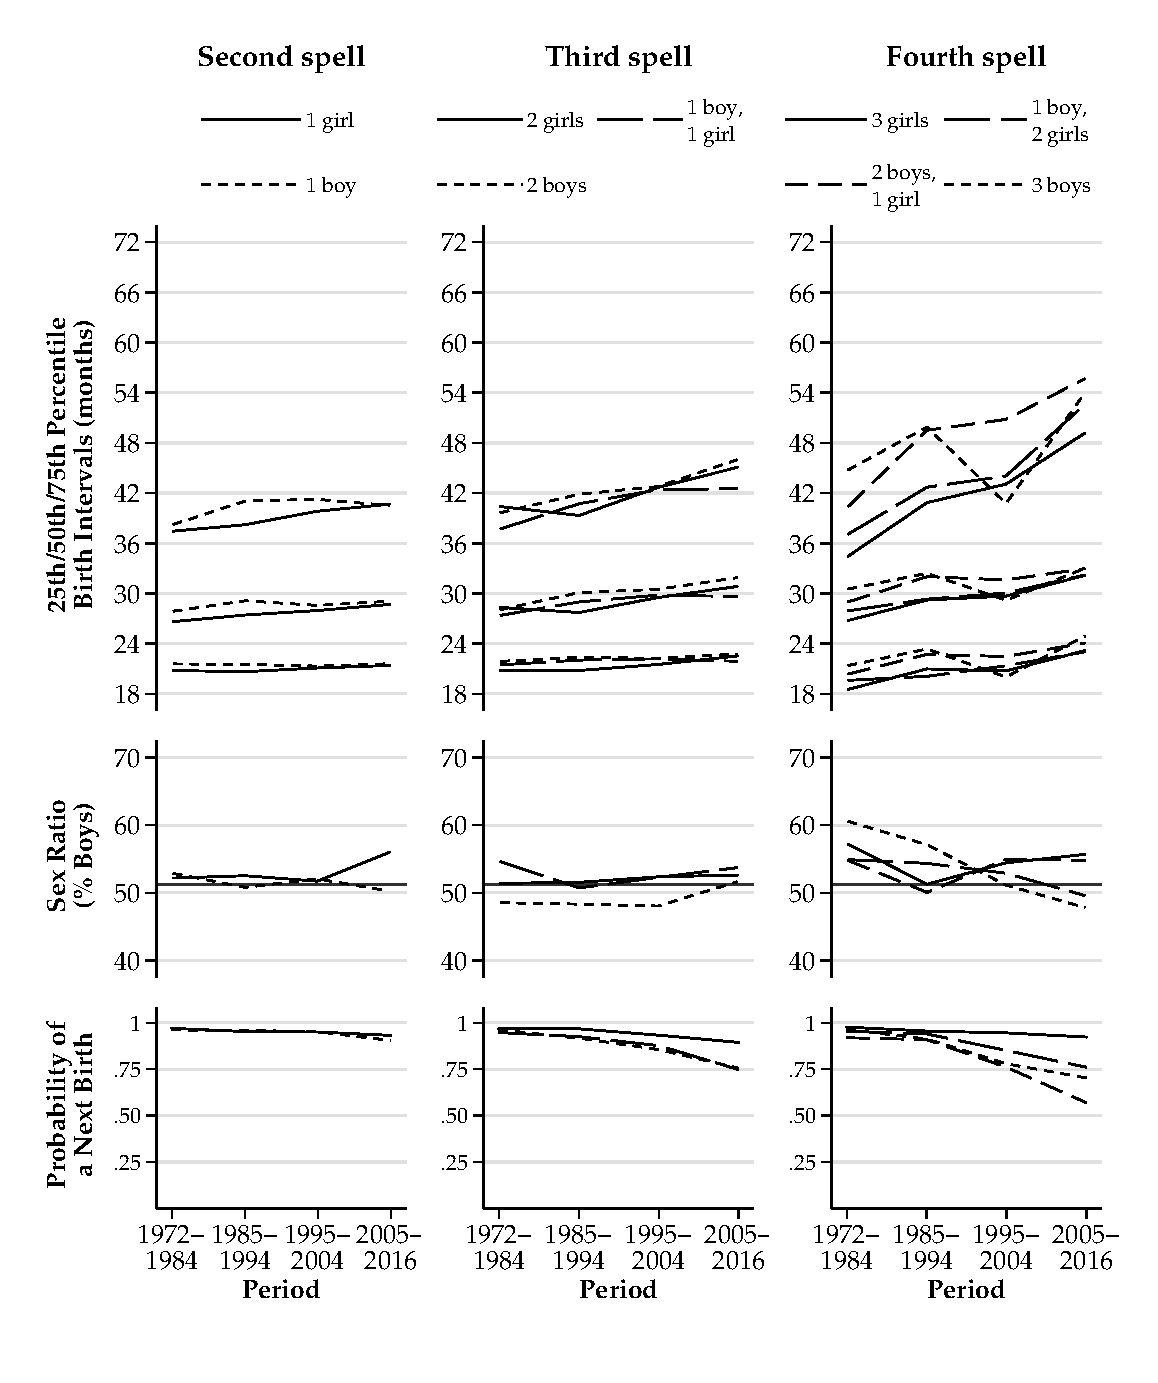
\includegraphics[width=\textwidth,height=\textheight,keepaspectratio=true]{bs_low_urban}
\caption{Percentile birth interval lengths, sex ratios, and parity progression  
for urban women with no education by spell, sex composition, and period}
\label{fig:spacing_low_urban}
\end{figure}

\begin{figure}
\centering
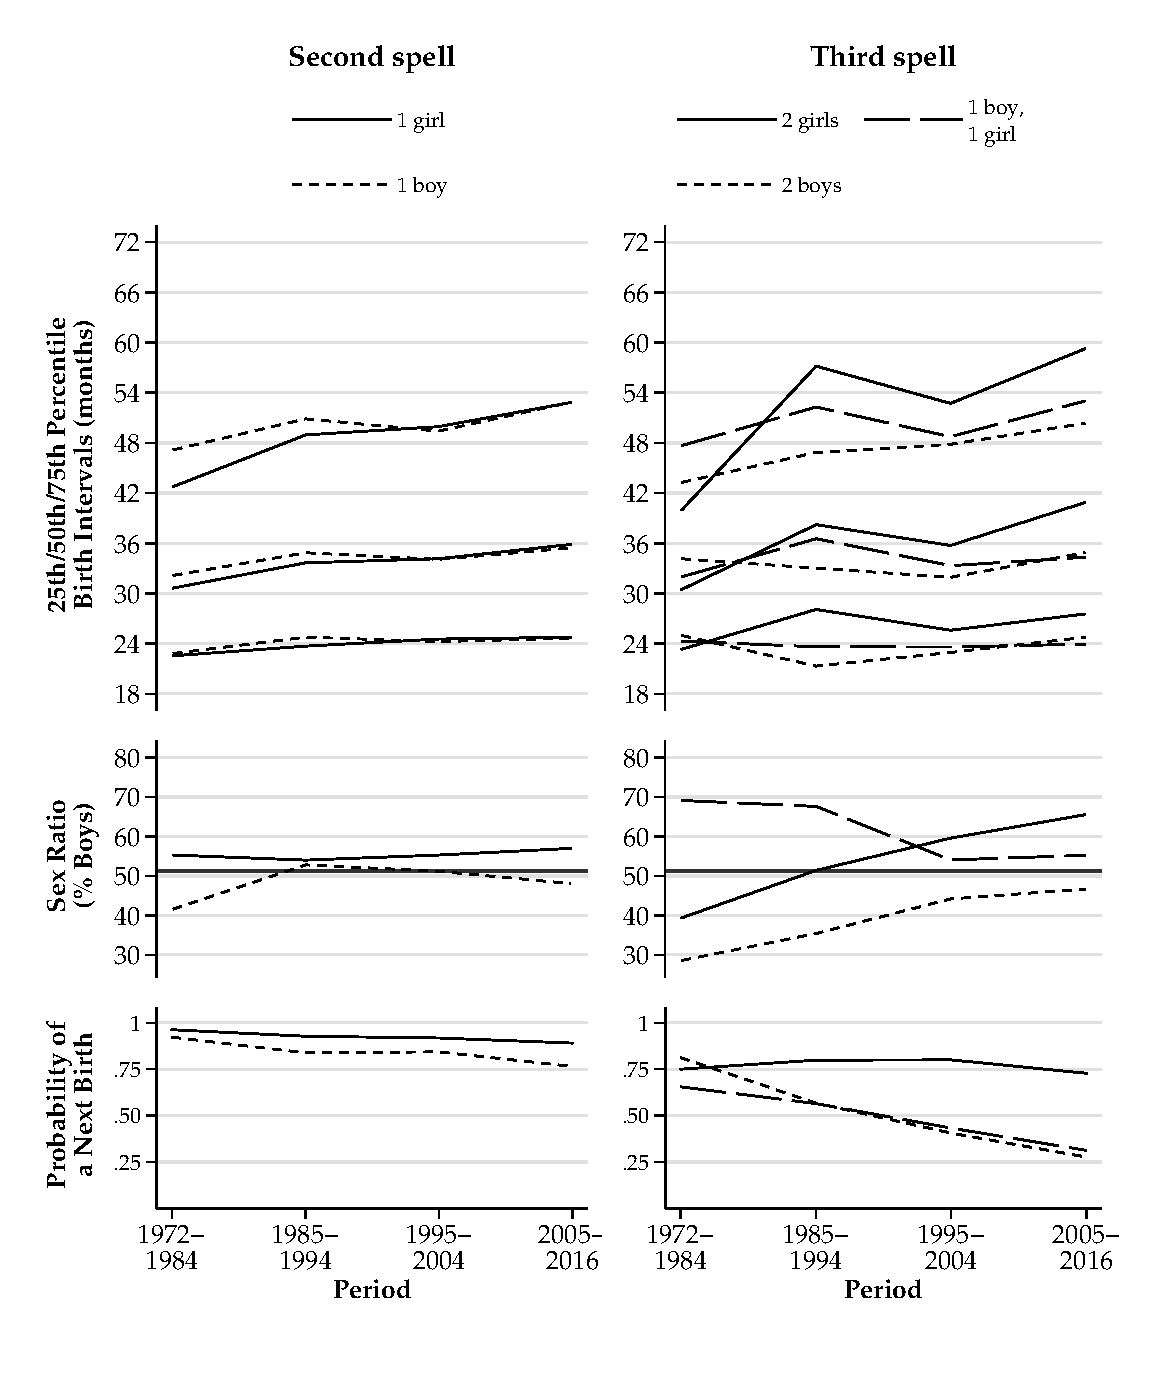
\includegraphics[width=\textwidth,height=\textheight,keepaspectratio=true]{bs_highest_rural}
\caption{Percentile birth interval lengths, sex ratios, and parity progression  
for rural women with 12 or more years of education by spell, sex composition, and period}
\label{fig:spacing_highest_rural}
\end{figure}



The first set of tables, Tables \ref{tab:p25_p50_p75_low}, \ref{tab:p25_p50_p75_med},
\ref{tab:p25_p50_p75_high}, and \ref{tab:p25_p50_p75_highest} show 25th, 50th, and
75th percentile birth interval lengths together with their standard errors.
The standard errors for all measures are based on bootstrapping,
where the model is repeatedly estimated using resampling with replacement.

The second set of tables, 
Tables \ref{tab:avg_sex_ratio_low}, \ref{tab:avg_sex_ratio_med}, 
\ref{tab:avg_sex_ratio_high}, and \ref{tab:avg_sex_ratio_highest}, show predicted average 
birth interval lengths, sex ratios, and probabilities of having a birth by decade, spell, and sex 
composition for the four education levels separated by the area of residence, together 
with bootstrapped standard errors for all three outcomes.
To find the average birth interval length, I calculate, for each woman, the probability of 
giving birth in each $t$, and her expected spell length from these probabilities. 
I then average the individual expected spell lengths across women using their parity 
progression probabilities as weights. Finally, I add nine months because spells begin 
nine months after the previous birth.

I also show whether durations for sex composition other than only girls are statistically 
significantly different from the duration with only girls based on bootstrapped 
differences. 
The cleanest test is comparing durations after only boys with durations after
only girls, but the number of births to women with only sons becomes small 
in the later periods.
Hence, it is possible to have substantial differences in spacing that are
not statistically significant because of low power, especially for the third 
and fourth spell.

Each predicted percent of boys is tested against the natural percentage of
boys using the bootstrapped standard errors.
The natural sex ratio is approximately 105 boys to 100 girls or
51.2\% \citep{jacobsen99,Portner2015b}.
The predicted percentage boys may differ from the natural rate because of 
natural variation, any remaining recall error not corrected for, or 
sex selection. 

\input{../tables/bootstrap_duration_p25_p75_low_all.tex}

\input{../tables/bootstrap_duration_p25_p75_med_all.tex}

\input{../tables/bootstrap_duration_p25_p75_high_all.tex}

\input{../tables/bootstrap_duration_p25_p75_highest_all.tex}

\input{../tables/bootstrap_duration_avg_sex_ratio_low_all.tex}

\input{../tables/bootstrap_duration_avg_sex_ratio_med_all.tex}

\input{../tables/bootstrap_duration_avg_sex_ratio_high_all.tex}

\input{../tables/bootstrap_duration_avg_sex_ratio_highest_all.tex}


\clearpage
\newpage


\section{Infant Mortality Graphs}

\setcounter{figure}{0}
\setcounter{table}{0}


\begin{figure}[!htp]
\centering
\includegraphics[width=0.8\textwidth,keepaspectratio=true]{mortality_spell_3_low_med}
\caption{Infant mortality by preceding birth interval length across periods for third child of women with 
no education and women with 1--7 years of education}
\label{fig:mortality_low_med_spell_3}
\end{figure}


\begin{figure}
\centering
\includegraphics[width=0.8\textwidth,keepaspectratio=true]{mortality_spell_3_high_highest}
\caption{Infant mortality by preceding birth interval length across periods for third child of women with 
8--11 and 12 and above years of education}
\label{fig:mortality_high_highest_spell_3}
\end{figure}


\clearpage

\onehalfspacing
\bibliographystyle{aer}
\bibliography{sex_selection_spacing}


\end{document}



